%\documentclass[table,xcolor=pdftex,dvipsnames]{beamer}
\documentclass[table,xcolor=pdftex,dvipsnames, handout]{beamer}\usepackage[]{graphicx}\usepackage[]{color}
%% maxwidth is the original width if it is less than linewidth
%% otherwise use linewidth (to make sure the graphics do not exceed the margin)
\makeatletter
\def\maxwidth{ %
  \ifdim\Gin@nat@width>\linewidth
    \linewidth
  \else
    \Gin@nat@width
  \fi
}
\makeatother

\definecolor{fgcolor}{rgb}{0.345, 0.345, 0.345}
\newcommand{\hlnum}[1]{\textcolor[rgb]{0.686,0.059,0.569}{#1}}%
\newcommand{\hlstr}[1]{\textcolor[rgb]{0.192,0.494,0.8}{#1}}%
\newcommand{\hlcom}[1]{\textcolor[rgb]{0.678,0.584,0.686}{\textit{#1}}}%
\newcommand{\hlopt}[1]{\textcolor[rgb]{0,0,0}{#1}}%
\newcommand{\hlstd}[1]{\textcolor[rgb]{0.345,0.345,0.345}{#1}}%
\newcommand{\hlkwa}[1]{\textcolor[rgb]{0.161,0.373,0.58}{\textbf{#1}}}%
\newcommand{\hlkwb}[1]{\textcolor[rgb]{0.69,0.353,0.396}{#1}}%
\newcommand{\hlkwc}[1]{\textcolor[rgb]{0.333,0.667,0.333}{#1}}%
\newcommand{\hlkwd}[1]{\textcolor[rgb]{0.737,0.353,0.396}{\textbf{#1}}}%
\let\hlipl\hlkwb

\usepackage{framed}
\makeatletter
\newenvironment{kframe}{%
 \def\at@end@of@kframe{}%
 \ifinner\ifhmode%
  \def\at@end@of@kframe{\end{minipage}}%
  \begin{minipage}{\columnwidth}%
 \fi\fi%
 \def\FrameCommand##1{\hskip\@totalleftmargin \hskip-\fboxsep
 \colorbox{shadecolor}{##1}\hskip-\fboxsep
     % There is no \\@totalrightmargin, so:
     \hskip-\linewidth \hskip-\@totalleftmargin \hskip\columnwidth}%
 \MakeFramed {\advance\hsize-\width
   \@totalleftmargin\z@ \linewidth\hsize
   \@setminipage}}%
 {\par\unskip\endMakeFramed%
 \at@end@of@kframe}
\makeatother

\definecolor{shadecolor}{rgb}{.97, .97, .97}
\definecolor{messagecolor}{rgb}{0, 0, 0}
\definecolor{warningcolor}{rgb}{1, 0, 1}
\definecolor{errorcolor}{rgb}{1, 0, 0}
\newenvironment{knitrout}{}{} % an empty environment to be redefined in TeX

\usepackage{alltt}

\usepackage{handoutWithNotes}
\pgfpagesuselayout{4 on 1 with notes}[letterpaper,border shrink=5mm]

\usepackage{beamerthemesplit}
\usepackage[english]{babel}
\usepackage{amsmath}
\usepackage{amssymb}
\usepackage{amsthm}
\usepackage{verbatim}
\usepackage{graphpap}
\usepackage{epic}
\usepackage{pict2e} %To draw line with any slope
\usepackage{color}
\usepackage{natbib}
\usepackage{enumitem}
\usepackage{booktabs}
\usepackage{xcolor}
\usepackage{soul}

\bibliographystyle{ajae}

\newcommand{\p}{\partial}

\newcommand {\framedgraphic}[1] {
        \begin{center}
            \includegraphics[width=\textwidth,height=0.7\textheight,keepaspectratio]{#1}
        \end{center}
        \vspace{-1\baselineskip}
}

\usetheme{Boadilla}
\useoutertheme{shadow}
\usecolortheme{beaver}%seagull
\everymath{\color{blue}}
\everydisplay{\color{blue}}

\usefonttheme{professionalfonts}

\usepackage{hyperref}
\hypersetup{
   colorlinks = {true},
   urlcolor = {blue},
   linkcolor = {black},
   citecolor = {black},
   pdfborderstyle={/S/U/W 1},
   urlbordercolor = 0 0 1,
   citebordercolor = 1 1 1,
   filebordercolor = 1 1 1,
   linkbordercolor = 1 1 1,
   pdfauthor = {Sebastien Pouliot}
}

\widowpenalty=10000 % Avoid single line at the end of a page
\clubpenalty=10000  % Avoid single line at the bottom

\title[Marketing margins]{Supply chains and marketing margins}
\author[Pouliot]{S\'{e}bastien Pouliot}
\institute{Iowa State University}
\date{Fall 2017}
\IfFileExists{upquote.sty}{\usepackage{upquote}}{}
\begin{document}

%%%%%%%%%%%%%%%%%%%%%%%%%%%%%%%%%%%%%%%%%%%%%%%%%%%%%%%%%%%%%%%%%%%%%%%%%%%%%%%%%%

\begin{frame}
\titlepage
\vspace{-0.4in}
\begin{center}
Lecture notes for Econ 235\\
\end{center}
\end{frame}

%%%%%%%%%%%%%%%%%%%%%%%%%%%%%%%%%%%%%%%%%%%%%%%%%%%%%%%%%%%%%%%%%%%%%%%%%%%%%%%%%%
\section[Introduction]{Introduction}

\begin{frame}{Definitions}
\begin{enumerate}[label=\textbullet]
  \item What is a \emph{marketing margin}?
      \begin{enumerate}[label=-]
          \item It is the difference between the price received by producers and the price paid by consumers.
      \end{enumerate}
  \item A similar measure is the \emph{farm value share}:
      \begin{enumerate}[label=-]
          \item It is the ratio of the price received by producers and the price paid by consumers.
      \end{enumerate}
\end{enumerate}
\end{frame}

%%%%%%%%%%%%%%%%%%%%%%%%%%%%%%%%%%%%%%%%%%%%%%%%%%%%%%%%%%%%%%%%%%%%%%%%%%%%%%%%%%


\begin{frame}{Definitions}
\begin{enumerate}[label=\textbullet]
  \item Some refer to a marketing margin as the \emph{price spread}.
  \item Why care about marketing margins?
      \begin{enumerate}[label=-]
          \item Concerns by producers and consumers over the size of margins and changes in the size of margins;
          \item Fear that the ``middleman" is taking advantage of its position;
          \item Are firms with market power capturing most of the value of a product?
          \item Why do marketing margins vary across products?
      \end{enumerate}
  \item Marketing margins are most meaningful for products that do not go through much transformation.
\end{enumerate}
\end{frame}


%%%%%%%%%%%%%%%%%%%%%%%%%%%%%%%%%%%%%%%%%%%%%%%%%%%%%%%%%%%%%%%%%%%%%%%%%%%%%%%%%%
\section{USDA data on price spread}

\begin{frame}{The USDA publishes data on price spread}
\begin{enumerate}[label=\textbullet]
  \item Information about food prices is available at: \url{http://www.ers.usda.gov/topics/food-markets-prices/food-prices-expenditures-costs.aspx}.
  \item Price spread data are available at: \url{http://www.ers.usda.gov/data-products/price-spreads-from-farm-to-consumer.aspx}.
  \item Food prices and spending at \url{http://www.ers.usda.gov/data-products/ag-and-food-statistics-charting-the-essentials/food-prices-and-spending.aspx}.
\end{enumerate}
\end{frame}

%%%%%%%%%%%%%%%%%%%%%%%%%%%%%%%%%%%%%%%%%%%%%%%%%%%%%%%%%%%%%%%%%%%%%%%%%%%%%%%%%%
\section{Marketing margins vary across time and across products}

\begin{frame}{Marketing margins for milk and dairy across time}
\begin{table}
\caption{Milk and dairy basket}
\tiny
\begin{tabular}{l c c c c}
  \toprule
  Year & \parbox[c]{0.6in}{\centering Retail cost} & \parbox[c]{0.6in}{\centering Farm value} & \parbox[c]{0.6in}{\centering Farm-to-retail spread} & \parbox[c]{0.6in}{\centering Farm value share} \\
  \cmidrule(r){2-5}
   & \multicolumn{3}{c}{2003=100} & Percent \\
  \midrule
  2000 & 96 & 97 & 95 & 28 \\
  2001 & 100 & 118 & 92 & 33 \\
  2002 & 100 & 95 & 102 & 27 \\
  2003 & 100 & 100 & 100 & 28 \\
  2004 & 107 & 128 & 99 & 33 \\
  2005 & 109 & 114 & 107 & 29 \\
  2006 & 108 & 101 & 111 & 26 \\
  2007 & 116 & 145 & 105 & 35 \\
  2008 & 125 & 145 & 118 & 32 \\
  2009 & 117 & 101 & 124 & 24 \\
  2010 & 119 & 127 & 115 & 30 \\
  2011 & 127 & 156 & 116 & 34 \\
  2012 & 129 & 143 & 124 & 31 \\
  2013 & 130 & 153 & 121 & 33 \\
  2014 & 134 & 185 & 115 & 38 \\
  2015 & 132 & 136 & 131 & 29 \\
  2016 & 129 & 130 & 129 & 28 \\
  \bottomrule
\end{tabular}
\end{table}
\end{frame}

%%%%%%%%%%%%%%%%%%%%%%%%%%%%%%%%%%%%%%%%%%%%%%%%%%%%%%%%%%%%%%%%%%%%%%%%%%%%%%%%%%

\begin{frame}{Marketing margins vary across commodities}
\begin{enumerate}[label=\textbullet]
  \item Have a look at these interactive charts \url{https://www.ers.usda.gov/data-products/price-spreads-from-farm-to-consumer/interactive-chart-price-spreads-and-food-markets/}.
\end{enumerate}
\begin{table}
\caption{Marketing margins across commodities in 2015}
\small
\begin{tabular}{l c c}
  \toprule
  Product & \parbox[c]{0.85in}{\centering Farm-to-retail spread (2001=100)} & \parbox[c]{0.85in}{\centering Farm value share} \\
  \midrule
   Milk and dairy basket & 131 &  29 \\
   Fresh fruit basket & 117 & 38 \\
   Fresh vegetables basket & 141 & 27 \\
   Flour, white, all purpose, per pound &  & 18 \\
  \bottomrule
\end{tabular}
\end{table}
\end{frame}


%%%%%%%%%%%%%%%%%%%%%%%%%%%%%%%%%%%%%%%%%%%%%%%%%%%%%%%%%%%%%%%%%%%%%%%%%%%%%%%%%%

\begin{frame}{What explains the difference in marketing margins?}
\begin{enumerate}[label=\textbullet]
  \item For commodities that are expensive to farm, the marketing margin will tend to be relatively small and the farm value share higher.
  \item The marketing margin is large and the farm value share is small for product that are substantially transformed.
\end{enumerate}
\end{frame}

%%%%%%%%%%%%%%%%%%%%%%%%%%%%%%%%%%%%%%%%%%%%%%%%%%%%%%%%%%%%%%%%%%%%%%%%%%%%%%%%%%

\begin{frame}{Marketing margins over time}
\begin{enumerate}[label=\textbullet]
  \item Reasons for changes in marketing margins over time:
     \begin{enumerate}[label=\arabic*.]
        \item Improvements in farming technologies has caused a decline in the cost of farming, thus causing a decline in the price of food commodities;
        \item Consumers demand more transformed products (e.g. ready to eat meals, food away from home). Processing of food occurs less at home;
        \item Marketing firms have been offering products that are increasingly more processed, thus increasing costs and the price paid by consumers. New technology facilitates the automation of the transformation of food.
     \end{enumerate}
  \item These three factors cause a decline in farm value share over time or equivalently, an increase in the marketing margin.
\end{enumerate}
\end{frame}

%%%%%%%%%%%%%%%%%%%%%%%%%%%%%%%%%%%%%%%%%%%%%%%%%%%%%%%%%%%%%%%%%%%%%%%%%%%%%%%%%%


\begin{frame}{Farm value share over time (1993-2014)}
\begin{knitrout}
\definecolor{shadecolor}{rgb}{0.969, 0.969, 0.969}\color{fgcolor}
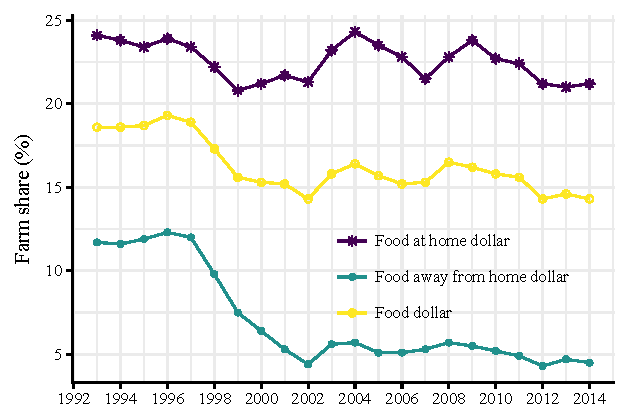
\includegraphics[width=\maxwidth]{figure/figure_farm_share-1} 

\end{knitrout}
\scriptsize
Note: The data are from \url{https://www.ers.usda.gov/data-products/food-dollar-series/download-the-data/}.
\end{frame}

%%%%%%%%%%%%%%%%%%%%%%%%%%%%%%%%%%%%%%%%%%%%%%%%%%%%%%%%%%%%%%%%%%%%%%%%%%%%%%%%%%
\section{What is the farm value share now}

\begin{frame}{Farm value share now}
\begin{enumerate}[label=\textbullet]
  \item The Economic Research Service (ERS) reports the \emph{Food Dollar Series}, which measures annual expenditures by U.S. consumers on domestically produced food.
  \item The Food Dollar Series is available online at: \url{http://www.ers.usda.gov/data-products/food-dollar-series.aspx}.
  \item There are three series in the Food Dollar Series:\emph{ marketing bill series}, \emph{the industry group series}, and \emph{the primary factors series}.
\end{enumerate}
\end{frame}

%%%%%%%%%%%%%%%%%%%%%%%%%%%%%%%%%%%%%%%%%%%%%%%%%%%%%%%%%%%%%%%%%%%%%%%%%%%%%%%%%%%%%

\begin{frame}{Marketing Bill series (2015)}
    \begin{center}
        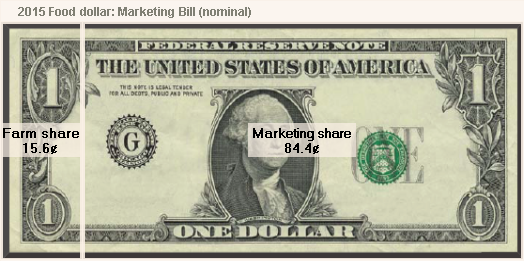
\includegraphics[width=0.75\textwidth,height=\textheight,keepaspectratio]{marketing_bill.png}
    \end{center}
    \vspace{-1\baselineskip}
\scriptsize
Source:  Food Dollar Series, available at: \url{http://www.ers.usda.gov/data-products/food-dollar-series.aspx}.
\end{frame}

%%%%%%%%%%%%%%%%%%%%%%%%%%%%%%%%%%%%%%%%%%%%%%%%%%%%%%%%%%%%%%%%%%%%%%%%%%%%%%%%%%%%%

\begin{frame}{Industry Group series (2015)}
    \begin{center}
        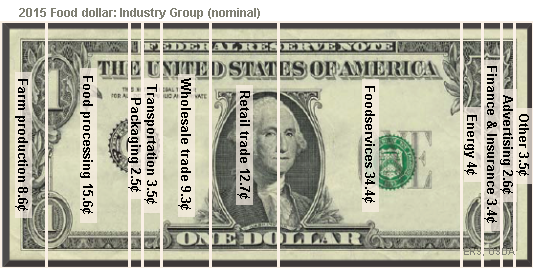
\includegraphics[width=0.75\textwidth,height=\textheight,keepaspectratio]{industry_group.png}
    \end{center}
    \vspace{-1\baselineskip}
\scriptsize
Source:  Food Dollar Series, available at: \url{http://www.ers.usda.gov/data-products/food-dollar-series.aspx}.
\end{frame}

%%%%%%%%%%%%%%%%%%%%%%%%%%%%%%%%%%%%%%%%%%%%%%%%%%%%%%%%%%%%%%%%%%%%%%%%%%%%%%%%%%%%%

\begin{frame}{Primary Factors series (2015)}
    \begin{center}
        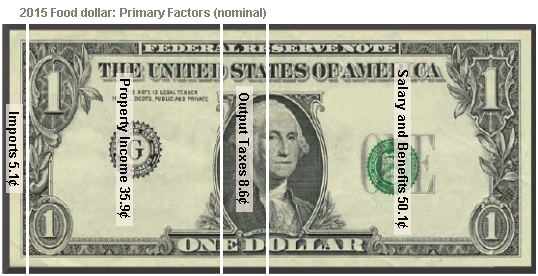
\includegraphics[width=0.75\textwidth,height=\textheight,keepaspectratio]{primary_factors.png}
    \end{center}
    \vspace{-1\baselineskip}
\scriptsize
Source:  Food Dollar Series, available at: \url{http://www.ers.usda.gov/data-products/food-dollar-series.aspx}.
\end{frame}


%%%%%%%%%%%%%%%%%%%%%%%%%%%%%%%%%%%%%%%%%%%%%%%%%%%%%%%%%%%%%%%%%%%%%%%%%%%%%%%%%%%%%
\section{Commodity prices and food prices}

\begin{frame}{Food prices and the 2012 drought}
\begin{enumerate}[label=\textbullet]
  \item The 2012 crop season started well for farmers in the Mid-West but the lack of rain quickly deteriorated growing conditions.
  \item Following the worst drought in 50 years, the 2012 harvest was disappointing, causing an increase in the price of agricultural commodities.
  \item What are the consequences of the drought on the price of food products?
\end{enumerate}
\end{frame}

%%%%%%%%%%%%%%%%%%%%%%%%%%%%%%%%%%%%%%%%%%%%%%%%%%%%%%%%%%%%%%%%%%%%%%%%%%%%%%%%%%%%%

\begin{frame}{How commodity prices affect the price of food?}
\begin{enumerate}[label=\textbullet]
  \item To see this, let's consider the example of a farrow-to-finish farm.
  \item We will use budgeting from Ag Decision Maker, prepared by extension economists here at Iowa State University: \url{http://www.extension.iastate.edu/agdm/livestock/html/b1-21.html}.
  \item On that webpage, open the decision aids excel file for \href{http://www.extension.iastate.edu/agdm/livestock/xls/b1-21farrowtofinishp6.xlsx}{farrow-to-finish}.
\end{enumerate}
\end{frame}

%%%%%%%%%%%%%%%%%%%%%%%%%%%%%%%%%%%%%%%%%%%%%%%%%%%%%%%%%%%%%%%%%%%%%%%%%%%%%%%%%%%%%

\begin{frame}{Farrow-to-finish production cost}
\begin{enumerate}[label=\textbullet]
  \item The excel sheet describes the cost of farrow-to-finish operation under reasonable assumptions about input quantities and their prices.
  \item The excel sheet differentiates between variable and fixed costs.
  \item Let's focus here on the variable cost. In particular, we will focus on the cost of corn feed, changing the value of the corn price and keeping everything else constant.
  \item As of \today, the price of corn in the excel sheet is \$3.30 per bushel.
  \item At that price, the break-even selling price for all costs is \$43.71 per cwt.
\end{enumerate}
\end{frame}

%%%%%%%%%%%%%%%%%%%%%%%%%%%%%%%%%%%%%%%%%%%%%%%%%%%%%%%%%%%%%%%%%%%%%%%%%%%%%%%%%%%%%

\begin{frame}{Break-even selling price for all costs?}
\begin{enumerate}[label=\textbullet]
  \item What's the meaning of the break-even selling price for all costs?
  \item It is the price of hog at which a farrow-to-finish operation exactly covers its costs.
  \item If the price of hog is greater than the break-even selling price, then a farrow-to-finish operation earns a profit. Otherwise it incurs a loss.
  \item Finishing hogs is a competitive business. Remember that \emph{economic profits} for competitive firms are zero in the long-run.
  \item The excel sheet shows a measure of \emph{accounting profit}.
\end{enumerate}
\end{frame}

%%%%%%%%%%%%%%%%%%%%%%%%%%%%%%%%%%%%%%%%%%%%%%%%%%%%%%%%%%%%%%%%%%%%%%%%%%%%%%%%%%%%%

\begin{frame}{Economic vs accounting profits}
\begin{enumerate}[label=\textbullet]
  \item The difference between economic and accounting profits is that economic profits include opportunity costs.
  \item The opportunity cost is the cost for not doing something else. It could be, for example, the cost of owning a hog finishing operation instead of owning a cattle feeding operation.
  \item For simplicity here, assume that economic profits equal accounting profit. That is, there is no opportunity cost of own a hog finishing operation.
\end{enumerate}
\end{frame}

%%%%%%%%%%%%%%%%%%%%%%%%%%%%%%%%%%%%%%%%%%%%%%%%%%%%%%%%%%%%%%%%%%%%%%%%%%%%%%%%%%%%%

\begin{frame}{Entry, exit and input costs}
\begin{enumerate}[label=\textbullet]
  \item In the long-run, entry and exit of farrow-to-finish operations will occur until profits equal zero, that is when the break-even selling price equals the market price.
  \item One implication is that at market equilibrium, changes in costs are reflected through changes in prices.
  \item That means that we can use the accounting sheet to study how an increase in the price of corn will impact the price of finished hogs in the long-run.
\end{enumerate}
\end{frame}


%%%%%%%%%%%%%%%%%%%%%%%%%%%%%%%%%%%%%%%%%%%%%%%%%%%%%%%%%%%%%%%%%%%%%%%%%%%%%%%%%%%%%

\begin{frame}{Effect of an increase in the price of corn}
\begin{enumerate}[label=\textbullet]
  \item Recall that at \$3.30 per bushel, the break-even price is \$43.71 per cwt.
  \item Suppose a 100\% increase in the price of corn, which thus increases to \$6.60 per bushel.
  \item At that new price of corn, the break-even price for all costs becomes \$59.96 per cwt.
  \item That is, for a 100\% increase in the price of corn, the price of hog should increase by about (59.96 - 43.71)/43.71 = 37\%.
  \item Why does the price of hog increases relatively less than the price of corn?
\end{enumerate}
\end{frame}


%%%%%%%%%%%%%%%%%%%%%%%%%%%%%%%%%%%%%%%%%%%%%%%%%%%%%%%%%%%%%%%%%%%%%%%%%%%%%%%%%%%%%

\begin{frame}{Effect of an increase in the price of corn}
\begin{enumerate}[label=\textbullet]
  \item The price of finished hogs increases proportionally less than the price of corn because the cost of corn is a fraction of the total cost of finishing hogs.
  \item From the excel sheet, the estimated cost of corn per litter when priced at \$3.30 per bushel is \$346.50.
  \item The total cost per litter is \$1,001.57.
  \item This means that at a price of \$3.30 per bushel, the cost share of corn is 34.6\% of the cost of finishing hogs.
  \item Thus, a 100\% increase in the price of corn causes roughly a 100\%*0.346=34.6\% increase in the price of hogs, close to the 37\% calculated before.
\end{enumerate}
\end{frame}

%%%%%%%%%%%%%%%%%%%%%%%%%%%%%%%%%%%%%%%%%%%%%%%%%%%%%%%%%%%%%%%%%%%%%%%%%%%%%%%%%%%%%

\begin{frame}{Is this change in the price of finished hogs correct?}
\begin{enumerate}[label=\textbullet]
  \item It understates the effect of an increase in the price of corn because:
    \begin{enumerate}[label=-]
        \item Corn is also an input in the production of gilts and boars;
        \item As soybean meal and DDGS are substitutes to corn, then an increase in the price of corn will cause increases in the prices of soybean meal and DDGS.
    \end{enumerate}
  \item It overstates the effect of an increase in the price of corn because:
    \begin{enumerate}[label=-]
        \item Farms can find substitutes to corn to use as a feed (candy?);
        \item Farms can adapt their production methods.
    \end{enumerate}
\end{enumerate}
\end{frame}

%%%%%%%%%%%%%%%%%%%%%%%%%%%%%%%%%%%%%%%%%%%%%%%%%%%%%%%%%%%%%%%%%%%%%%%%%%%%%%%%%%%%%

\begin{frame}{Going all the way up the supply chain}
\begin{enumerate}[label=\textbullet]
  \item Even if the numbers calculated in the previous slides are not exactly accurate, what we learn from them is that an increase in the price of one input will tend to have a small impact on the price of an output because the cost of a single input is typically a small share of the total costs.
  \item Going all the way up the supply chain to pork purchased by consumer, the cost share of corn will become very small.
  \item Suppose that the cost share of live hogs to packing houses is 0.5 and that the cost share of marketing pork meat all the way up to sales at retail is 0.5, then this means that in total, corn represents about 34.6\%*0.5*0.5=8.65\% of the cost of pork at retail.
\end{enumerate}
\end{frame}

%%%%%%%%%%%%%%%%%%%%%%%%%%%%%%%%%%%%%%%%%%%%%%%%%%%%%%%%%%%%%%%%%%%%%%%%%%%%%%%%%%%%%

\begin{frame}{Going all the way up the supply chain}
\begin{enumerate}[label=\textbullet]
  \item With these numbers, it means that an increase in the price of corn by 100\%, would cause an increase in the price of pork by only 8.65\%.
  \item Farm commodity prices account for only a small fraction of the cost of food at retail.
  \item This is also true for many products other than pork.
  \item Any change in commodity prices has a small impact on food prices at retail.
  \item This is true only for food products and are transformed. For instance, an orange is the same at the farm and at the consumer level.
\end{enumerate}
\end{frame}

%%%%%%%%%%%%%%%%%%%%%%%%%%%%%%%%%%%%%%%%%%%%%%%%%%%%%%%%%%%%%%%%%%%%%%%%%%%%%%%%%%

\begin{frame}{In practice, the effect is even smaller...}
\begin{enumerate}[label=\textbullet]
  \item The examples in the previous slide assume that the commodities enter in a fixed proportion in the food product.
  \item For many food products, the assumption that a commodity enters in a fixed proportion in the production of a food product is not true.
  \item For producers and manufacturers, it is often possible to substitute one input by another.
  \item For example, \href{http://money.cnn.com/2012/10/10/news/economy/farmers-cows-candy-feed/index.html}{cash-strapped farmers feed candy to cows.}
  \item Another example is the use of high-fructose corn syrup instead of cane sugar in the production of soda (pop!) in the United States.
\end{enumerate}
\end{frame}

%%%%%%%%%%%%%%%%%%%%%%%%%%%%%%%%%%%%%%%%%%%%%%%%%%%%%%%%%%%%%%%%%%%%%%%%%%%%%%%%%%

\begin{frame}{In practice, the effect is even smaller...}
\begin{enumerate}[label=\textbullet]
  \item Thus, unless food-makers are constrained by a recipe, they will substitute expensive ingredients (inputs) with less expensive ingredients as much as they can.
  \item In economics, the ability to substitute an input by another is measured by the elasticity of substitute $\sigma$.
  \item If $\sigma=0$, then firms are not able to substitute one input for another.
  \item For $\sigma>0$, then firms are able substitute inputs.
  \item For $\sigma \rightarrow \infty$, inputs are perfect substitute. High-fructose corn syrup and cane sugar are close to being perfect substitutes.
\end{enumerate}
\end{frame}

%%%%%%%%%%%%%%%%%%%%%%%%%%%%%%%%%%%%%%%%%%%%%%%%%%%%%%%%%%%%%%%%%%%%%%%%%%%%%%%%%%%%%

\begin{frame}{About the 2012 drought and food prices}
\begin{enumerate}[label=\textbullet]
  \item Huge increase in the price of commodities.
  \item What happened to the price of food? Not much!
  \item USDA predicts price for food.
  \item \href{http://www.youtube.com/watch?v=6IZdRqzFed8&list=FLA-0GE7G6Acb_YRgztz-BrQ&index=9}{Drought Affecting Food Prices In 2013 - USDA video on YouTube}.
  \item Consistent with the previous discussion, USDA predicted a small impact of the drought on food prices.
\end{enumerate}
\end{frame}

%%%%%%%%%%%%%%%%%%%%%%%%%%%%%%%%%%%%%%%%%%%%%%%%%%%%%%%%%%%%%%%%%%%%%%%%%%%%%%%%%%%%%

\begin{frame}{Drought in California}
\begin{figure}[htbp]
\caption{U.S. drought monitor for California in November 2015}
    \framedgraphic{drought_California.png}
\end{figure}
\scriptsize
Source: \url{http://droughtmonitor.unl.edu/CurrentMap/StateDroughtMonitor.aspx?CA}.
\end{frame}

%%%%%%%%%%%%%%%%%%%%%%%%%%%%%%%%%%%%%%%%%%%%%%%%%%%%%%%%%%%%%%%%%%%%%%%%%%%%%%%%%%%%%

\begin{frame}{Drought in California}
\begin{figure}[htbp]
\caption{U.S. drought monitor for California in November 2016}
    \framedgraphic{drought_California_2016.png}
\end{figure}
\scriptsize
Source: \url{http://droughtmonitor.unl.edu/CurrentMap/StateDroughtMonitor.aspx?CA}.
\end{frame}


%%%%%%%%%%%%%%%%%%%%%%%%%%%%%%%%%%%%%%%%%%%%%%%%%%%%%%%%%%%%%%%%%%%%%%%%%%%%%%%%%%%%%

\begin{frame}{Drought in California}
\begin{figure}[htbp]
\caption{U.S. drought monitor for California in November 2017}
    \framedgraphic{drought_California_2017.png}
\end{figure}
\scriptsize
Source: \url{http://droughtmonitor.unl.edu/CurrentMap/StateDroughtMonitor.aspx?CA}.
\end{frame}


%%%%%%%%%%%%%%%%%%%%%%%%%%%%%%%%%%%%%%%%%%%%%%%%%%%%%%%%%%%%%%%%%%%%%%%%%%%%%%%%%%%%%

\begin{frame}{What about the effect of the current drought}
\begin{enumerate}[label=\textbullet]
  \item California is a large producer of fruits, vegetables, tree nuts and dairy.
  \item \href{http://www.c-span.org/video/?318343-5/washington-journal-factors-impact-us-food-prices}{Factors that impact U.S. food prices} on C-SPAN. The video is a bit long but very informative.
  \item The idea is the same as before, if the cost of an input represents a small share of the cost at retail, then an increase in the price at the farm has a small impact on the price at retail.
  \item For those less processed products, the change in prices will occur faster.
  \item For fresh fruits and vegetables, imports helped buffer the effect of the California drought.
  \item More information available at: \url{http://usda.proworks.com/topics/in-the-news/california-drought-farm-and-food-impacts/california-drought-food-prices-and-consumers/}.
\end{enumerate}
\end{frame}


%%%%%%%%%%%%%%%%%%%%%%%%%%%%%%%%%%%%%%%%%%%%%%%%%%%%%%%%%%%%%%%%%%%%%%%%%%%%%%%%%%%%%

\begin{frame}{What about eggs?}
\begin{enumerate}[label=\textbullet]
  \item Iowa and other US States have been affected by an outbreak of avian influenza in the spring of 2015.
  \item This caused a significant decline in the production of eggs in Iowa and in other states.
  \item Eggs produced in Iowa are mostly for breaking to make liquid and powdered eggs.
  \item Still, the events associated with avian influenza outbreak impact shell eggs at retail because of demand and supply substitution.
\end{enumerate}
\end{frame}

%%%%%%%%%%%%%%%%%%%%%%%%%%%%%%%%%%%%%%%%%%%%%%%%%%%%%%%%%%%%%%%%%%%%%%%%%%%%%%%%%%%%%

\begin{frame}{Retail vs wholesale egg prices}
\begin{figure}[htbp]
\caption{Large white egg prices in \$ per dozen}
    \framedgraphic{Egg_retail_wholesale.png}
\end{figure}
\end{frame}

%%%%%%%%%%%%%%%%%%%%%%%%%%%%%%%%%%%%%%%%%%%%%%%%%%%%%%%%%%%%%%%%%%%%%%%%%%%%%%%%%%%%%

\begin{frame}{Are eggs sold at a loss?}
\begin{enumerate}[label=\textbullet]
  \item The margin between retail and wholesale was on average pretty stable until Spring 2015.
  \item The margin was reduced significantly with the increase in the price of eggs caused by the avian flu.
  \item It is possible that eggs are retail are sold at a loss over a short period of time, especially during holidays.
  \item The margin returned to its normal value but seems to have been very small recently, possibly negative.
\end{enumerate}
\end{frame}


%%%%%%%%%%%%%%%%%%%%%%%%%%%%%%%%%%%%%%%%%%%%%%%%%%%%%%%%%%%%%%%%%%%%%%%%%%%%%%%%%%%%%

\section{From the consumers to farms}

\begin{frame}{From consumers to farms}
\begin{enumerate}[label=\textbullet]
  \item What about asking the question the other way around?
  \item How does a change in the demand (e.g. the demand shifts out) for a food product affect the price of agricultural commodities?
\end{enumerate}
\end{frame}

%%%%%%%%%%%%%%%%%%%%%%%%%%%%%%%%%%%%%%%%%%%%%%%%%%%%%%%%%%%%%%%%%%%%%%%%%%%%%%%%%%%%%

\begin{frame}{From consumers to farms}
\begin{enumerate}[label=\textbullet]
  \item As there are many factors of production (inputs) in a supply chain (e.g. agricultural commodity, trucking, refrigeration, storage, labor...), a change in the price of a food product will affect the price of all of these factors of production.
  \item Only when the supply of a factor of production is perfectly elastic that its price does not change.
  \item The sign of the change in the price of other inputs is the same as the change in the price of the output.
  \item For inputs that are inelastically supplied:
        \begin{enumerate}[label=-]
          \item Large changes in prices;
          \item Small changes in quantities.
        \end{enumerate}
  \item For inputs that are elastically supplied:
        \begin{enumerate}[label=-]
          \item Small changes in prices;
          \item Large changes in quantities.
        \end{enumerate}
\end{enumerate}
\end{frame}

%%%%%%%%%%%%%%%%%%%%%%%%%%%%%%%%%%%%%%%%%%%%%%%%%%%%%%%%%%%%%%%%%%%%%%%%%%%%%%%%%%%%%

\begin{frame}{From consumers to farms}
\begin{enumerate}[label=\textbullet]
  \item The value shares of inputs also matter:
        \begin{enumerate}[label=-]
          \item The prices and the quantities of inputs that have small value share change by less.
        \end{enumerate}
  \item The elasticity of substitutions also matter:
        \begin{enumerate}[label=-]
          \item Stronger effect on prices and quantities of inputs that do not have substitutes.
        \end{enumerate}
  \item Thus, the effect of a change in the demand for a food product is distributed through a supply chain according to the supply elasticities of inputs, the elasticities of substitution and the values shares.
  \item This means that the farm price may see only a small effect of an increase in the demand for a food product.
\end{enumerate}
\end{frame}

%%%%%%%%%%%%%%%%%%%%%%%%%%%%%%%%%%%%%%%%%%%%%%%%%%%%%%%%%%%%%%%%%%%%%%%%%%%%%%%%%%%%%

\begin{frame}{Other information}
\begin{enumerate}[label=\textbullet]
  \item If you want to learn the complexity of the food supply chain, you can look at data from the input-output matrix from the \href{http://www.bea.gov/newsreleases/industry/io/2013/io1213.htm}{Bureau of Economic Analysis}.
  \item People at Tuft University have a prepared a \href{http://usfoodpolicy.blogspot.com/search/label/visualization}{tool} to visualize those data
\end{enumerate}
\end{frame}



%%%%%%%%%%%%%%%%%%%%%%%%%%%%%%%%%%%%%%%%%%%%%%%%%%%%%%%%%%%%%%%%%%%%%%%%%%%%%%%%%%%%%
%\section{References}
%\renewcommand\refname{References}
%\def\newblock{References}
%\begin{frame}[allowframebreaks]{References}
%\bibliography{D:/Dropbox/Papers/References}
%\bibliography{C:/Users/pouliot/Documents/Papers/References}
%\end{frame}


%%%%%%%%%%%%%%%%%%%%%%%%%%%%%%%%%%%%%%%%%%%%%%%%%%%%%%%%%%%%%%%%%%%%%%%%%%%%%%%%%%%%%

\end{document}

